\documentclass[a4paper,10pt, oneside]{article}
\usepackage[utf8]{inputenc}
\usepackage[T1]{fontenc}
\usepackage[spanish]{babel}
\usepackage[style=ieee,backend=bibtex]{biblatex}
\usepackage{graphicx}
\usepackage{amsmath}
\usepackage{pgfplots}
\usepackage{lineno}
%\usepackage{showframe}
\usepackage[top=1in, bottom=1.25in, left=1.25in, right=1.25in]{geometry}
\usepackage{caption}
\usepackage{bytefield}
\usepackage{amsmath}
\usepackage{csquotes}
\usepackage{svg}
\usepackage{lscape}
\usepackage{multicol}
\usepackage{subfig}
\usepackage{hyperref}



\usepackage{listings,xcolor}
\lstset{
	string=[s]{"}{"},
	stringstyle=\color{blue},
	comment=[l]{:},
	commentstyle=\color{black},
}


\bibliography{informe_2}

	
\begin{document}
	
\begin{titlepage}
	\centering
	
\includegraphics[width=0.25\textwidth]{../../Universidad_del_Litoral}\par\vspace{1cm}
	{\scshape\LARGE Universidad Nacional del Litoral \par}
	\vspace{1cm}
	{\scshape\Large Proyecto Final de Carrera\par}
	\vspace{1.5cm}
	{\huge\bfseries Diseño de un sistema de detección de anomalías en redes de computadoras.\par}
	\vspace{4cm}
	{\huge\bfseries Informe de avance 2\par}
	\vfill
	
	{\Large \itshape Pineda Leandro\par}
	
	
	% Bottom of the page
	\large Córdoba\par
	{\large \today\par}	
\end{titlepage}

\modulolinenumbers[5]
\linenumbers

\section{Introducción}
Determinar anomalías en una serie temporal de eventos permite detectar fenómenos que pueden ser de interés para ciertas aplicaciones. Por ejemplo, monitorear la demanda de recursos en un servicio de red, o determinar que anuncio publicitario es la más visto en un sitio web.

Es interesante observar anomalías en el comportamiento de ciertos componentes en distintos puntos de una red de datos. Por ejemplo, pueden analizarse los flujos de datos en los puntos de acceso de la red. En la capa de transporte, el protocolo TCP (que provee conexión host a host sobre IP) provee información suficiente para identificar estos patrones. Además, los diferentes servicios que funcionan en una red, como servidores web, producen grandes cantidades de registros de auditoría (o logs) que pueden ser analizado en busca de patrones anómalos.
Para llevar a cabo el análisis en tiempo real de eventos (tanto los segmentos TCP que son transportados como los logs de los distintos servicios o eventos generados por cierta aplicación), utilizaremos el modelo de \textit{data streaming}: este se basa esencialmente en algoritmos que procesan una única vez los datos, dado que transferirlos y almacenarlos no es posible en la práctica, y permiten determinar cuales son los elementos más comunes en el stream de datos, así como algunos estadísticos (como la media, mediana, histograma), entre otros.

\section{El modelo de data streaming}

En este modelo, las entradas que van a ser procesadas no están disponibles para ser accedidas aleatoriamente desde disco o memoria, sino que llegan como uno o mas flujos continuos de datos. Los \textit{streams} de datos son diferentes de los modelos relacionales convencionales\footnote{Datos en almacenados usando un gestor de base de datos} en varios aspectos: 
\begin{itemize}
	\item Los elementos del stream deben ser procesados de manera \textit{online}.
	\item Los sistemas que procesan los datos no tienen control sobre el orden en los elementos de la entrada.
	\item Los stream de datos pueden ser infinitos.
	\item Una vez que un elemento es procesado, este se descarta.\footnote{En algunas aplicaciones los elementos pueden ser almanacenados para ser procesados posteriormente, pero en un modelo de streaming "puro" los elementos son procesados una única vez.}
\end{itemize}

Con respecto a los datos podemos hacer una distinción entre \textit{consultas únicas} y \textit{consultas continuas}\cite{Terry:1992:CQO:141484.130333}. Las consultas únicas (como aquellas que se hacen mediante un DBMS tradicional) son evaluadas una vez sobre un \textit{snapshot} de un conjunto de datos. La consultas continuas, por otro lado, son evaluadas continuamente mientras el \textit{stream} de datos esta siendo procesado. Las respuestas a estas consultas pueden ser almacenadas y actualizadas en la medida que llegan nuevos flujos de datos, o pueden ser origen de otro \textit{stream} de datos.

Para el análisis de tráfico de red, podemos pensar a los flujos TCP que pasan por un \textit{gateway} como los eventos o \textit{keys} a ser procesados. Las \textit{keys} pueden ser agrupadas mediante la 5-tupla dirección de IP de origen, destino, número de puerto de origen y destino y protocolo. De esta manera se puede analizar el comportamiento del tráfico de red de cada una de las sesiones en busca de anomalías como ser sesiones que hacen uso intensivo de recursos de red en un momento del tiempo. Sin embargo, el espacio de las \textit{keys} es tan grande que llevar registro de todos los eventos no es viable. Este tipo de problemas y similares llevaron al desarrollo de los llamados \textit{modelos de streaming} y la utilización de diferentes técnicas de conteo: bajo esta abstracción, los algoritmos procesan la entrada una única vez y deben calcular de manera precisa varios resultados usando recursos (espacio y tiempo por elemento) de forma estrictamente sublineal al tamaño de la entrada\cite{Muthukrishnan:2005:DSA:1166409.1166410}. Existen diferentes algoritmos para procesar y obtener información acerca de los eventos usando estructuras de datos que utilizan el espacio de memoria eficientemente. Sin embargo, estos métodos no calculan la frecuencia exacta de cada evento sino que la estiman: en general, para cantidades masivas de eventos basta con tener una buena aproximación de las frecuencias para identificar anomalías.

El problema de los eventos frecuentes consiste en procesar una serie consecutiva de elementos y encontrar aquellos que ocurren más frecuentemente en un período de tiempo. Es un problema muy estudiado en la minería de \textit{streams} de datos debido a que la resolución de muchos problemas se basan directa o indirectamente en la identificación de eventos frecuentes.

Los algoritmos para encontrar elementos frecuentes pueden dividirse en dos clases. Aquellos basados en técnicas de conteo llevan registro de un subconjunto de elementos y monitorean los contadores asociados con los mismos. Por cada entrada nueva, el algoritmo decide si guardar el elemento o no, y con que valor hacerlo. Por otro lado, los algoritmos basados en \textit{sketchs} realizan proyecciones lineales aleatorias de las entradas\cite{Cormode:2008:FFI:1454159.1454225} (vistas como vectores de características) y por lo tanto, no almacenan explícitamente los elementos de entrada. Estos últimos tienen ciertas propiedades que son de gran utilidad para procesamiento de múltiples \textit{streams} de datos.

\section{Detección de anomalías}
Cómo se mencionó anteriormente, determinar eventos frecuentes puede dar indicios de ciertos escenarios. Una práctica muy común en la etapa reconocimiento\footnote{El modelo de seguridad informática llamado \textit{cyber kill chain} describe las 7 etapas que todo atacante ejecuta para lograr su objetivo.\cite{hutchins2011intelligence}}, es el escaneo de puertos; uno o varios atacantes envían paquetes a un rango de puertos para determinar que servicios están activos, generando así grandes volúmenes de tráfico en la red. Otro escenario crítico es el de \textit{command and control (C2)} en donde el atacante tiene control de un conjunto de equipos ya infectados y utiliza sus recursos para atacar otro objetivo. Esto también genera tráfico anómalo y es un indicador crítico ante el cual se deben tomar medidas inmediatamente. Otro indicador son las fluctuaciones repentinas en los flujos de datos, que pueden indicar ataques de denegación de servicio (DoS).

La lista de ataques podría extenderse, pero de forma general pueden definirse dos tipos de comportamientos anómalos que son útiles para identificar amenazas. A continuación se describe el modelo de \textit{data streaming} y se definen los tipos de comportamiento anómalo.


\subsection{Modelado del problema}\label{modelado}

Consideremos un conjunto de eventos consecutivos o \textit{stream} de eventos donde cada evento es representado usando una tupla $(x, v_x)$. El elemento $x$ pertenece a un dominio $T=\{0,1,2, \dots, n-1\}$ con $|T|=n$, y $v_x$ es un valor asociado a $x$. El valor $v_x=1$ representa cantidad de eventos identificados por $x$. Definimos \textbf{\textit{heavy hitters}} como aquellos elementos que aparece más frecuentemente en el \textit{stream} de eventos. Los \textbf{\textit{heavy changers}} son aquellos elementos que presentan inconsistencias significativas entre el comportamiento observado y el comportamiento normal del flujo de datos (el cual se basa en lo ocurrido en el pasado) en un período de tiempo acotado\cite{Tong:2016:HTS:2927964.2927977}. 
En un algoritmo de detección de \textbf{\textit{heavy keys}}\footnote{Este término suele utilizase para referirse a ambos tipos de anomalías} típicamente se realizan dos procedimientos: en el de actualización el valor de cada elemento es procesado y se almacenan los resultados en una estructura de datos intermedia; en el de detección se examina la estructura de datos en cada época y se determinan los \textit{heavy keys}.

Para detectar \textit{heavy keys} se realizan estimaciones de frecuencias en ventanas de tiempo o épocas. En cada época, sea $S(x)$ la suma de los valores $v_x$ del elemento $x$. Sea $D(x)$ la diferencia (en valor absoluto) de $S(x)$ en la época actual y la anterior. Además, sea $U=\sum_{x \in T} S(x)$ la suma total de todos los elementos $x$ en una época. El problema de detectar \textit{heavy keys} consiste en encontrar aquellos elementos cuya suma o diferencias excedan, en valor absoluto, al parámetro $\phi$ en una época. Formalmente, definimos cómo \textit{heavy hitters} a aquellos elementos $x$ con $S(x) \geq \phi_1$, y \textit{heavy changers} a los elementos $x$ con $D(x) \geq \phi_2$. En adelante, referiremos indistintamente a los parámetros $\phi_1$ y $\phi_2$ como $\phi$, teniendo en cuenta que pueden ser diferentes.

\section{Métodos para determinar elementos frecuentes}

La forma clásica de procesar grandes volúmenes de datos y obtener información relevante asume que la totalidad de los datos están almacenados y pueden ser consultados en cualquier orden. Otro enfoque utiliza herramientas del \textit{data streaming} basadas en algoritmos livianos sumamente eficientes (sublineales en el uso de memoria), y estructura de datos probabilistas que pueden usarse para responder ciertas preguntas sobre los datos, de manera precisa y con una probabilidad razonablemente alta. Es decir, en lugar de almacenar la totalidad de los datos para se procesados, se utiliza una representación simplificada de los mismos.

Los \textit{sketch} son estructuras de datos que pueden ser pensadas como proyecciones lineales de los datos de entrada. Si representamos las entradas como vectores, estos pueden ser multiplicados por una \textit{matriz sketch}. El \textit{vector sketch} resultado contiene la  información suficiente para responder de forma aproximada ciertas preguntas sobre los datos. Por ejemplo, si codificamos los elementos de un \textit{stream} de datos como vectores cuya $i$-ésima entrada es su frecuencia $f_i$, el \textit{sketch} es el producto de este vector y una matriz: existen diferentes formas de definir la \textit{matriz sketch}, cada una con aplicaciones particulares. Para conteo de eventos se usan familias de funciones de \textit{hash} con ciertas propiedades para definir la proyección lineal.

Los algoritmos basados en \textit{sketches} resuelven el problema de estimación de frecuencia, pero necesitan información adicional para resolver el problema de los elementos frecuentes. Por esto, se suele aumentar la estructura de datos de los \textit{sketch} con algún método de conteo para encontrar elementos frecuentes de manera eficiente\footnote{Dos algoritmos conocidos son usualmente referidos como Majority y Frequent.}.

\

Antes de describir los algoritmos basados en \textit{sketches} es conveniente introducir los filtros \textit{Bloom}, que son una versión simplificada de los primeros, para ganar intuición acerca del funcionamientos de estas estructuras de datos.

\subsection{Filtros Bloom}

El término \textit{filtro Bloom} refiere a una estructura de datos compacta que se usa para representar conjuntos. Sin embargo, no es un conjunto ordinario dado que puede reportar falsos positivos cuando se consulta por la existencia de cierto elemento \cite{Putze:2010:CHS:1498698.1594230}.

\begin{figure}[htbp]
	\centering
	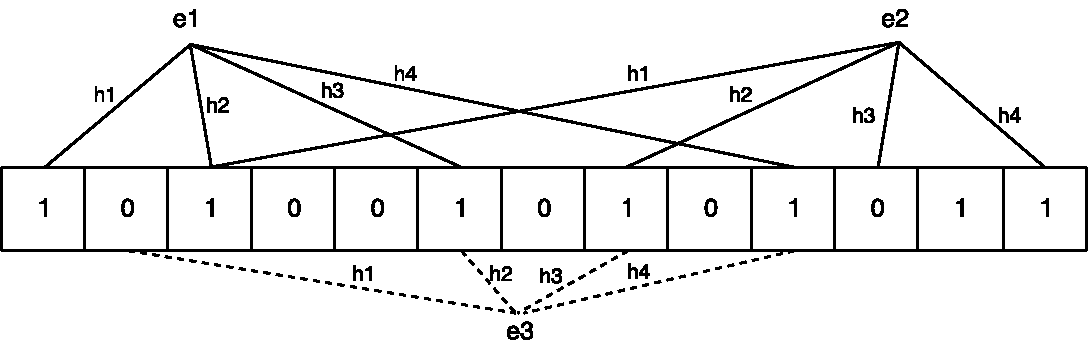
\includegraphics[scale=0.8]{graph/bloomFilter.pdf}
	\caption{Filtro Bloom}
	
	\medskip
	\small
	
	\parbox{13.1cm}{La imagen muestra un filtro de Bloom luego que los elementos $e_1$ y $e_2$ fueron insertados. Podemos observar que $e_3$ no es parte del conjunto dado que al menos uno de los bits en la posición que indican las funciones de hash es $0$. La pertenencia de un elemento cualquiera $e'$ al conjunto puede ser reportada erróneamente si las $k$ funciones de hash $h_i(e')$ apuntan a bits del filtro con valor $1$.}
	
\end{figure}

La ventaja principal de esta estructura de datos sobre las tradicionales es la eficiencia en el uso de memoria. Para representar un conjunto de a lo sumo $n$ elementos, un \textit{filtro Bloom} clásico hace uso de un vector de $m$ bits. Al comienzo todos los bits están en $0$. Para insertar un elemento $e$ en el filtro, $k$ bits son actualizados en base a la evaluación de $k$ funciones de hash independientes $h_1(e)$, $h_2(e)$, \dots, $h_k(e)$. Para consultar si un elemento es parte del conjunto se deben calcular las $k$ funciones de hash. Si todos los bits que indican las funciones de hash están en $1$ es probable que el elemento sea parte del conjunto, de lo contrario es seguro que el elemento no forma parte del conjunto. Sea $c=m/n$, la elección óptima para $k$ está dada por $k=int(\ln 2 \ c) = int(\ln 2 \ m/n)$ y la probabilidad de obtener un falso positivo (en promedio) está dada por $f_{std} (m,n,k) \approx (1-e^{-kn/m})^k$\cite{Bloom:1970:STH:362686.362692}. Por ejemplo, para un universo de $n=65536$ elementos y usando $c=4$ bits por elemento tenemos que $f_{std}=0.0174$.


\subsection{CountMin Sketch}

Los \textit{sketches} son menos populares que los \textit{filtros Bloom} pero comparten ciertas similitudes. Son estructuras de datos que permiten sumarizar un \textit{stream} de datos y pueden utilizarse para resolver el problema de los elementos frecuentes. Esto puede ser llevado a cabo usando menos espacio del que se utilizaría almacenando un contador por elemento, pero permitiendo que los contadores tengan cierto error en algunas ocasiones.

El \textit{sketch} COUNTMINT\cite{Cormode:2005:IDS:1073713.1073718} se utiliza para sumarizar \textit{streams} de datos. Consiste en un arreglo de $d \times w$ contadores y $d$ funciones de hash independientes $h_j$ con $1<j<d$ que mapean un elemento $i$ a un entero $z \in \{0, 1, \dots w-1\}$. Por cada elemento procesado se actualiza $d$ contadores en la posición $(j,h_j(i))$ (uno por cada fila) incrementando su valor en $1$.

\begin{figure}[htbp]
	\centering
	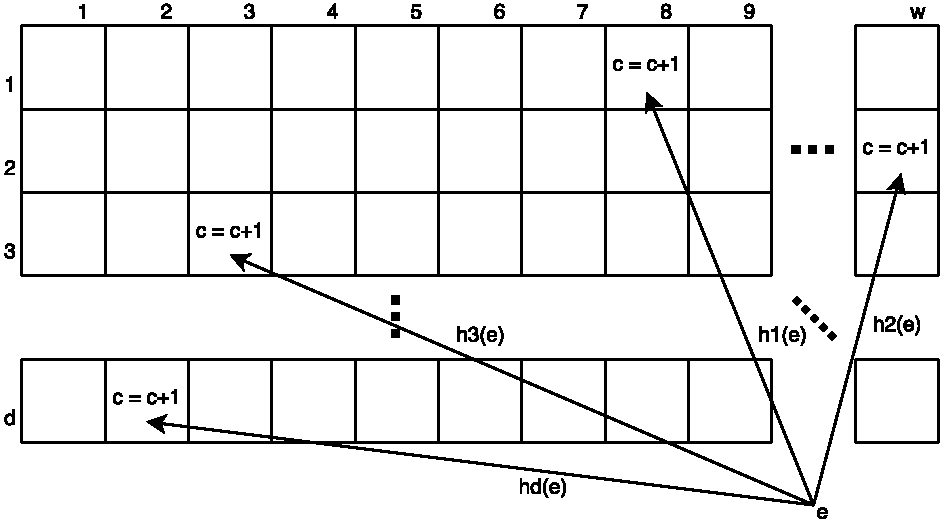
\includegraphics[width=0.6\textwidth]{graph/cmSketch.pdf}
	\caption{CountMin Sketch}
	\label{fig:cmSketch}
\end{figure}


Sea $\mathbf{a}$ un vector de frecuencias, de dimensión $n$, cuyo estado en el tiempo $t$ es $\mathbf{a}(t)=[a_1(t), a_2(t), \dots, a_n(t)]$. Inicialmente $\mathbf{a}$ es el vector $\mathbf{0}$, es decir $a_i(0)=0 \ \forall i$. Las actualizaciones a los elementos de $\mathbf{a}$ se representan mediante un \textit{stream} de tuplas. De forma general, la tupla $(i_t, c_t)$ representa el $t$-ésimo elemento procesado:\footnote{Para conteo de elementos $c_t=1$.}

\begin{gather*}
a_{i_t}(t)=a_{i_t}(t-1) + c_t\\
a_{i_{t'}}(t)=a_{i_{t'}}(t-1) \ \forall t' \neq t 
\end{gather*}

Usando \textit{sketches} podemos estimar la frecuencia de ocurrencia $a_i$ de un elemento $i$ mediante la fórmula $\hat{f_i} = min_{1 \leq j \leq d}\{C[j,h_j(i)]\}$. Se puede demostrar que $a_i \leq \hat{f_i}$ y que $\hat{f_i} \leq a_i + \varepsilon ||\mathbf{a}||_1$ con probabilidad mayor o igual a $1-\delta$. Los parámetros $\varepsilon$ y $\delta$ definen las dimensiones del \textit{sketch} como $w=\lceil \frac{e}{\varepsilon}\rceil$ y $d=\lceil \ln \frac{1}{\delta} \rceil$.

\paragraph{Ejemplo} Para procesar 10 millones de eventos y producir estimaciones con un error hacia arriba menor o igual a $100$ con una probabilidad de al menos $0.99$ necesitamos $\varepsilon ||\mathbf{a}||_1=100$ y $\delta = 0.01$. En términos las dimensiones del \textit{sketch} $w=271829$ y $d=5$.

\

Finalmente, COUNTMIN es $O({1 \over \epsilon} \log {1 \over \delta})$ en términos de memoria y para realizar operaciones de actualización es $O(\log {1 \over \delta})$

\section{Primer incremento: detección local de anomalías}
Se diseñó y se implementó un \textit{webservice} que expone los recursos necesarios para actualizar las estructuras de datos según el modelo descrito (de forma transparente para el usuario) y monitorear los evento detectados por el sistema. Estos últimos son representados usando un \textit{string} de longitud variable, pudiendo así adaptarse a cualquier uso, y son almacenados en una base de datos central de tipo \textit{clave-valor}. Este diseño permite usar un modelo en el que cada evento se representa mediante un número entero, y asociar a este una cadena de caracteres que de semántica a dicho valor (es decir, el evento). En general, los eventos son logs de subsistemas, pero pueden ser cualquier cadena de caracteres. Por supuesto, esta asociación número-\textit{string} se implementa de tal forma que si la misma cadena de caracteres aparece $n$ veces, siempre se le asigna el mismo valor numérico, dando así unicidad a la asociación. La detección de eventos ocurre automáticamente en intervalos de tiempo regulares y se mantiene un historial de los eventos detectados. La configuración del tamaño de las estructuras de datos, los parámetros de detección y el intervalo de detección pueden ser modifican mediante un archivo de configuración.
La implementación que será descrita a continuación puede encontrarse en  \url{https://github.com/leandropineda/sketch-ws/releases/tag/report2}.

\subsection*{Implementación}

El estado del \textit{sketch} se actualiza ejecutando una API REST por cada evento que se quiere ingresar al \textit{webservice}. El cuerpo de la consulta es de tipo \textit{application/json}\cite{rfc4627}: contiene el \textit{string} que representa el evento. Si bien en términos de performance esta no es la implementación más eficiente, proveer una interfaz REST para dialogar con el servicio hacer que el sistema pueda ser integrado en cualquier aplicación existente de manera sencilla. 

\

El objeto \textit{sketchManager} es el encargado de crear y actualizar los \textit{sketches}. Cada nuevo evento se asocia a un número entero, que luego es utilizado para actualizar el \textit{sketch}, mediante \textit{RedisManager}. Finalmente, la respuesta del recursos es el valor al que el evento fue asociado. El diagrama de secuencia se muestra en la figura \ref{fig:SecDiagResourceAddEvent}.

\begin{figure}[htbp]
	\centering
	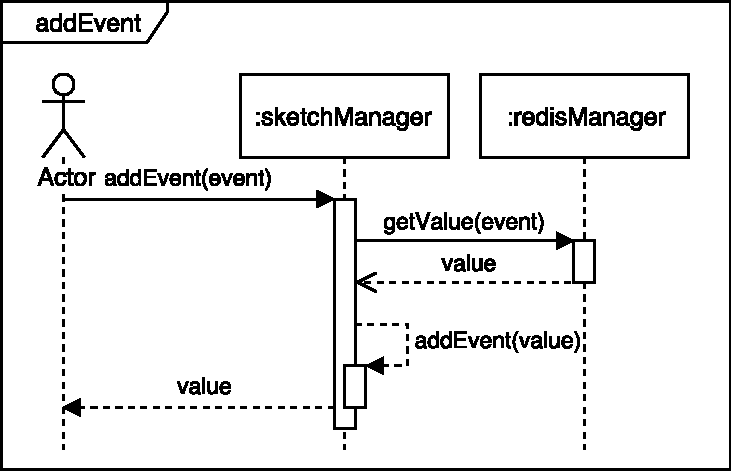
\includegraphics[width=0.45\textwidth]{graph/SecDiag-resourceAddEvent.pdf}
	\caption{Diagrama de secuencia para nuevos eventos}
	\label{fig:SecDiagResourceAddEvent}
\end{figure}

La asociación de una valor numérico a los eventos se respalda con una base de datos \textit{clave-valor}. El método \textit{getOrSet(event)} es el encargado de proveer el valor asociado al evento. Si no existe en la base de datos, se obtiene un valor para ser asociado al nuevo evento y se guardan el par \textit{<evento, valor>} y su inverso \textit{<valor, evento>} en la base de datos. Finalmente se retorna el valor asociado al evento.

En la figura \ref{fig:RedisManagerGetValue} se muestra el diagrama de secuencia para la asociación de un valor a los eventos:

\begin{figure}[htbp]
	\centering
	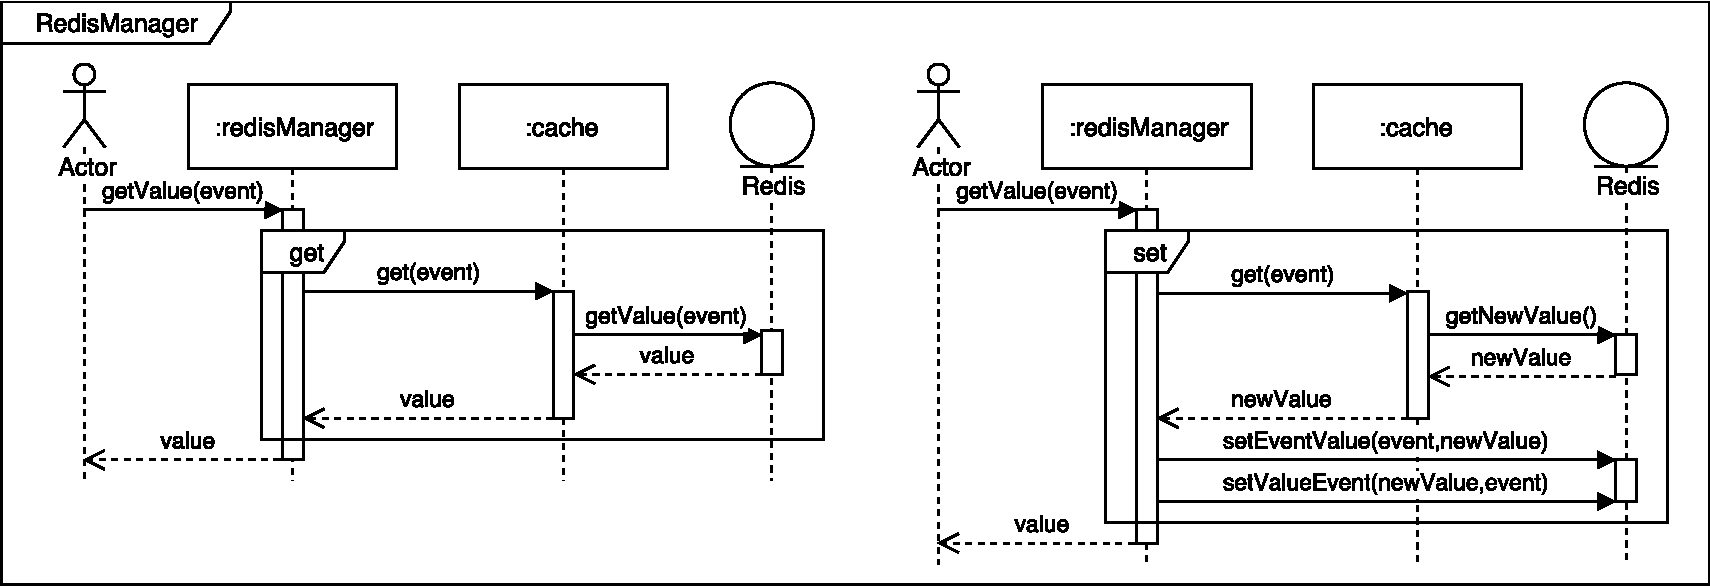
\includegraphics[width=1\textwidth]{graph/SecDiag-redisManagerGetValue.pdf}
	\caption{Diagrama de secuencia del flujo de acceso a la base de datos.}
	\label{fig:RedisManagerGetValue}
	
\end{figure}

Como las consultas a la base de datos usualmente son costosas y generan retrasos (es decir, introducen latencia), se colocó una \textit{cache} en el acceso a la base de datos. Con este diseño se busca solucionar los siguientes problemas:
\begin{itemize}
	\item Disminuir la carga de procesamiento del \textit{microservicio}: es mucho más eficiente operar con valores enteros que con cadenas de caracteres.
	\item Los algoritmos de \textit{streaming} están basados en funciones de \textit{hashing} y por lo tanto hacen uso intensivo de aritmética de enteros.
	\item Ante un escenario de detección distribuida, permite homogeneizar los eventos usando un repositorio centralizado, como una base de datos.
\end{itemize}


Para realizar la detección de \textit{heavy keys} se necesitan dos \textit{sketches} adyacentes en el tiempo. El mecanismo de rotación de \textit{sketches} está encapsulado en la clase \textit{SketchManager} y se implementa utilizando una \textit{cache} de un objeto que añade el \textit{sketch} activo a \textit{SketchHistory} cada vez que se invalida el mismo. El flujo descrito se puede observar en el diagrama de secuencia de la figura \ref{fig:SecDiagDetectionSchedulerRotation}.

\begin{figure}[htbp]
	\centering
	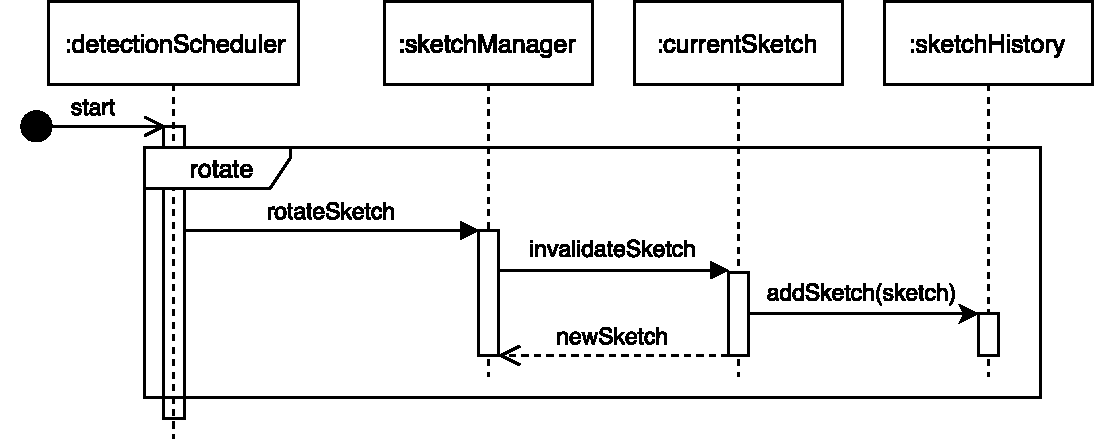
\includegraphics[width=0.8\textwidth]{graph/SecDiag-detectionSchedulerRotation.pdf}
	\caption{Diagrama de secuencia para la rotación de \textit{sketches}.}
	\label{fig:SecDiagDetectionSchedulerRotation}
\end{figure}

Para realizar la detección de \textit{heavy keys} la clase \textit{HeavyKeyDetector} usa los 2 últimos \textit{sketches} disponibles en \textit{sketchHistory}. Dado que los resultados de los algoritmos de detección son valores numéricos, es necesario obtener los eventos a los que fueron asociados previamente. Esta transformación es realizada por \textit{RedisManager}. Finalmente, \textit{HeavyKeyDetector} agrega a \textit{HeavyKeyDetectionHistory} los resultados de la detección son puestos a disposición del usuario mediante recursos en una API REST.

\begin{figure}[htbp]
	\centering
	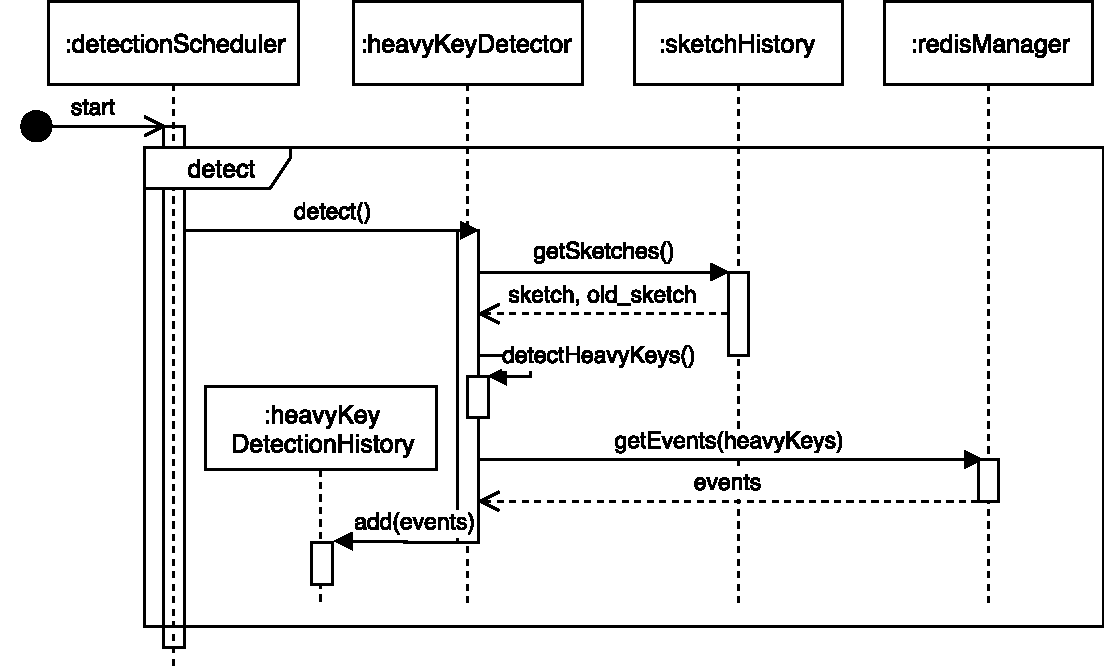
\includegraphics[width=0.8\textwidth]{graph/SecDiag-detectionSchedulerDetect.pdf}
	\caption{Diagrama de secuencia para detección de \textit{heavy keys}.}
	\label{fig:SecDiagDetectionSchedulerDetect}
\end{figure}

La implementación descrita esta empaquetada usando contenedores Docker\footnote{https://www.docker.com/}, y todas los componentes necesarios para su funcionamiento así como su configuración están definidas en un archivo \textit{docker-compose}. Estos contenedores permiten empaquetar software en unidades estandarizadas agilizando el desarrollo y puesta en producción de las aplicaciones. El \textit{webservice} provee además los recursos REST para consultar el estado del servicio y sus dependencias.

\section{Pruebas realizadas}

Se realizaron dos experimentos para comprobar el funcionamiento del servicio. En el primero se generaron una serie de eventos en el tiempo con un patrón en particular. En el segundo experimento se utilizaron los flujos TCP/IP de una captura de tráfico de red para generar los eventos generados por un equipo de red. 

\subsection{Patrones de eventos generados localmente}
Para el primer experimento se generaron una serie de eventos consecutivos en el tiempo, representados como un par \textit{(tiempo, evento)}. Para cada etiqueta, los eventos son espaciados regularmente en el intervalo de tiempo en el que se generaron, y se agregan pequeñas perturbaciones para evitar que la cantidad de eventos en ventanas adyacentes sea idéntica. Además, se agregan una serie de eventos aleatorios para simular situaciones reales donde pueden existir otras etiquetas que introducen ruido a la señal.

En la figura \ref{fig:prueba1} se observa la distribución de los eventos generados a lo largo del tiempo, para un intervalo de 60 segundos. Cada barra del gráfico representa un intervalo de tiempo de $3$ segundos.
Los eventos se generan para los intervalos de tiempo definidos de la siguiente manera: en el intervalo $(0,10)$ se generan $1200$ eventos $E1$, en $(10,40)$ se generan $800$ eventos $E2$, en $(33,36)$ se generan $400$ eventos $E3$, en $(40,47)$ se generan $500$ eventos $E4$ y en $(54,58)$ se generan $400$ eventos $E5$. Finalmente se suman $1500$ eventos aleatorios a toda la duración de la simulación. 

\begin{figure}[ht]
	\centering
	\makebox[0pt][c]{%
		\begin{minipage}{0.75\textwidth}
			\centering
			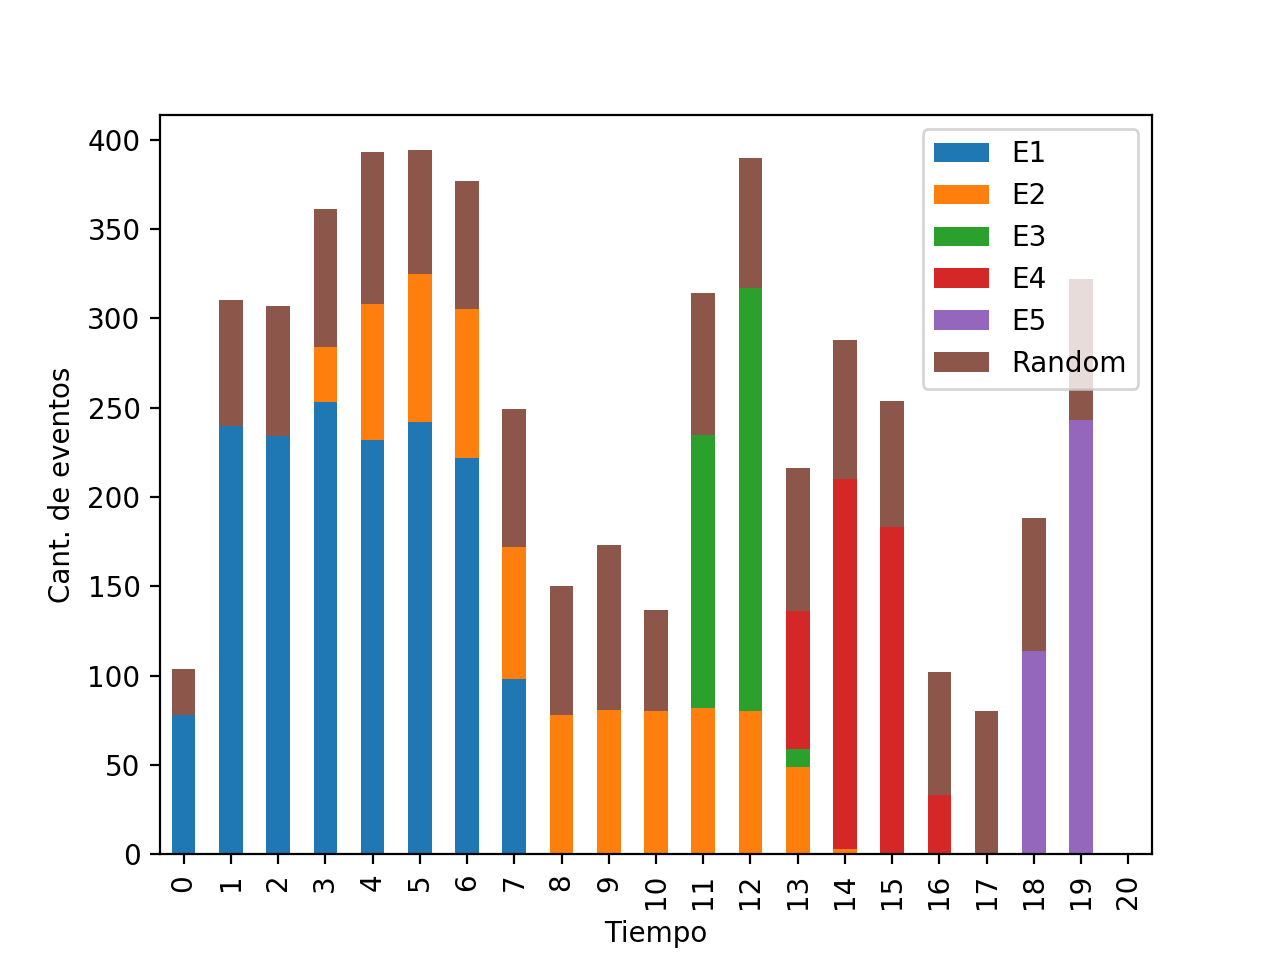
\includegraphics[scale=0.7]{graph/prueba1.png}
			\caption{Distribución de los eventos en el tiempo}
			\label{fig:prueba1}
		\end{minipage}
		\begin{minipage}{0.6\textwidth}
			\small
			\centering
			\begin{tabular}{ | l | c | c | c | c | c | c | c | c |}			
				\hline			
				Tiempo & 0 & 1 & 2 & 3 & 4 & 5 & 6 \\
				\hline
				Heavy Hitters & - & E1 & E1 & E1 & E1 & E1 & E1\\
				Heavy Changers & E1 & - & - & - & - & - & - \\
				\hline
				\hline
				Tiempo & 7 & 8 & 9 & 10 & 11 & 12 & 13  \\
				\hline
				Heavy Hitters & E1 & - & - & - & - & E3 & - \\
				Heavy Changers & E1 & - & - & - & E3 & E3 & E3 \\
				\hline\hline
				Tiempo & 14 & 15 & 16 & 17 & 18 & 19 & 20 \\
				\hline
				Heavy Hitters & - & E4 & E4 & - & - & E5 & - \\
				Heavy Changers & E4 & - & E4 & - & E5 & E5 & - \\
				\hline
			\end{tabular}
			\caption{HeavyKeys detectadas}
			\label{tab:prueba1}
		\end{minipage}
	}%
\end{figure}

Comprobando los resultados de la detección, se puede observar un defasaje entre los eventos detectados y los mostrados en la figura \ref{fig:prueba1}. Esto es así debido a que la simulación no inicia necesariamente en el comienzo de una época de detección (es decir, al comienzo de la ventana de tiempo de $3$ segundos configurada para este experimento). Por ejemplo, $E1$ es reportado como \textit{heavy changer} al momento $0$ cuando en realidad debería pasar inadvertido. Sin embargo, en el siguiente intervalo es reportado correctamente.
De la misma manera, podemos ver que el evento $E2$ no es reportado dado que esta por debajo de los límites configurados.

\

Los parámetros con los que el servicio estaba configurado a la hora de realizar esta prueba son: 

\begin{multicols}{2}
	\begin{itemize}
		\item Sketches
		\begin{itemize}
			\item rows(5)
			\item cols(100)
			\item prime(7283)
		\end{itemize}
	\end{itemize}
	\columnbreak
	\begin{itemize}
		\item Detección
		\begin{itemize}
			\item heavyHitterThreshold(150)
			\item heavyChangerThreshold(100)
			\item sketchRotationInterval(3)
		\end{itemize}
	\end{itemize}
\end{multicols}

\subsection{Trafico de red}
En esta prueba se utilizó un archivo de captura de tráfico de red para emular el comportamiento de los paquetes que atraviesan una interfaz de red. Este dataset, que es usado en la suite \textit{Tcpreplay\footnote{http://tcpreplay.appneta.com/wiki/captures.html}} para probar performance en switches y adaptadores de red, esta diseñado para generar una gran cantidad de flujos usando varios protocoles, manteniendo bajo el tráfico promedio de la red. Contiene 15000 paquetes de red y una duración de 300 segundos.

\begin{figure}[h!]
	\centering
	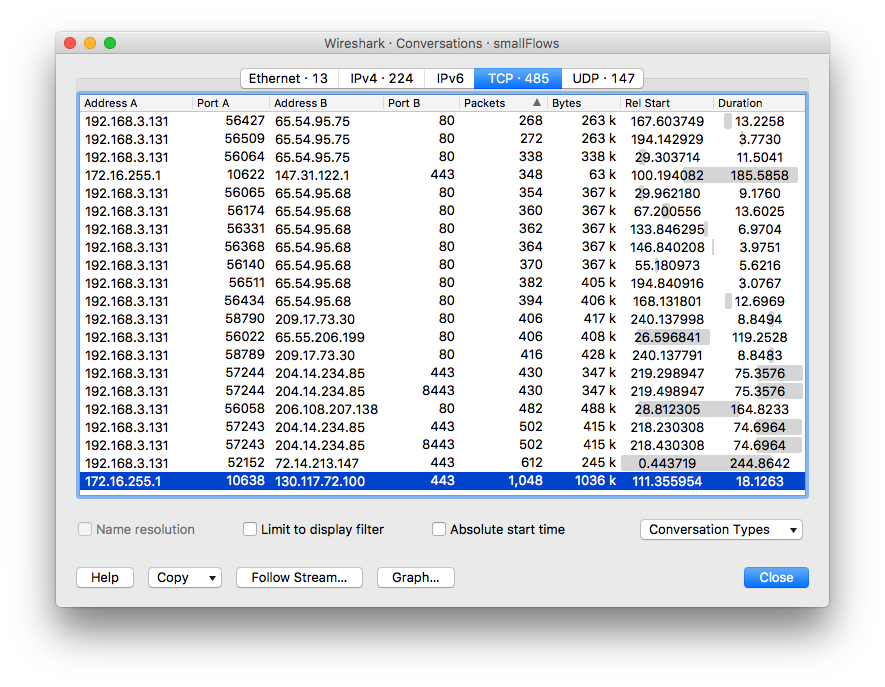
\includegraphics[width=.9\textwidth]{graph/smallFlows_conversations.png}
	\caption{Conversaciones TCP del archivo de captura de tráfico de red}
	\label{fig:smallFlows_conversation}
	
\end{figure}

Analizando los flujos que se muestran en la figura \ref{fig:smallFlows_conversation} se puede observar que la conversación con mayor cantidad de paquetes ocurre entre las direcciones 130.117.72.100:443 y 172.16.255.1:10638. A partir del instante $111.35$ se intercambian $1048$ paquetes en un período de $18.12$ segundos, que son detectados correctamente como \textit{heavy changers}. Los parámetros con los que se configuró el sistema son similares a los usados en el experimento anterior, solo que se aumentaron los umbrales: \textit{heavyHitterThreshold} es $250$ y \textit{heavyChangerThreshold} es $200$.


\section{Conclusión y trabajos futuros}
Para un flujo de eventos representados como cadenas de caracteres el sistema permite identificar en tiempo real aquellos eventos considerados como \textit{heavy keys} (ver \ref{modelado}). Codificando los eventos de esta manera el sistema puede ser integrado en diferentes aplicaciones sin dificultad, dado que expone interfaces sencillas.

Respecto a la instalación del sistema vemos que no ofrece dificultad alguna dado que esta diseñado como un microservicio. Los contenedores Docker funcionan en cualquier sistema operativo y pueden desplegarse tanto en infraestructura \textit{on-prem} como en el \textit{cloud}.

Es posible modificar las propiedades de los parámetros de detección del sistema usando un archivo de configuración según los datos que se quieren procesar. Los umbrales de detección deben ser configurados acorde a la aplicación, pero podría implementarse un mecanismo de ajuste automático.

Finalmente, dado que una REST API no es eficiente para el manejo de muchas peticiones, no se pueden utilizar grande volúmenes de eventos. Para esto, es necesario reemplazar el mecanismo REST por un \textit{message broker} como \textit{Apache ActiveMQ} e implementar el la lógica necesaria para soportar concurrencia en todos los módulos del sistema.


\newpage

\nocite{*}
\printbibliography
\end{document}

